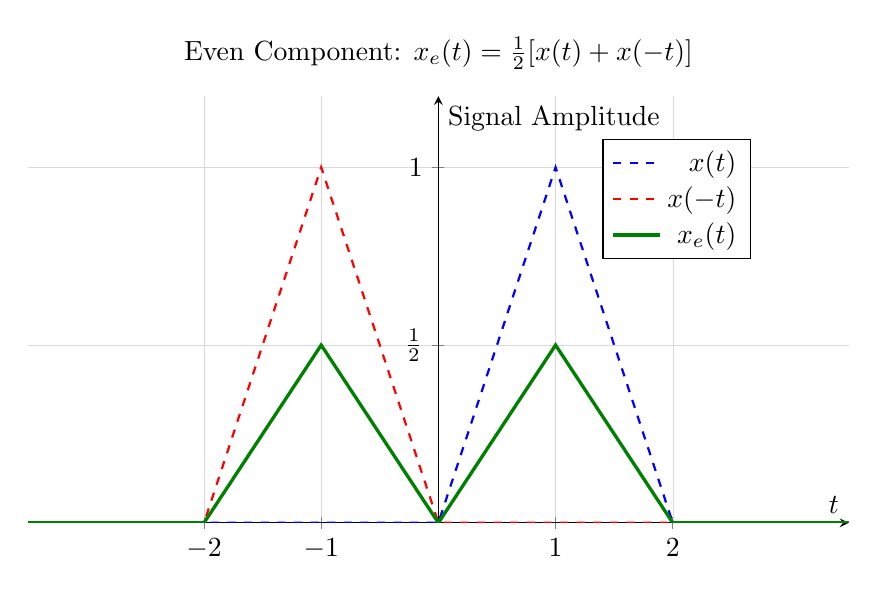
\begin{tikzpicture}
	\begin{axis}[
		% Set the overall style
		width=12cm,
		height=7cm,
		% Title with the definition of the even component
		title={Even Component: $x_e(t) = \frac{1}{2}[x(t) + x(-t)]$},
		% Axis labels
		xlabel={$t$},
		ylabel={Signal Amplitude},
		% Position axes at the origin
		axis lines=middle,
		% Set axis limits to show all signals
		xmin=-3.5, xmax=3.5,
		ymin=0, ymax=1.2,
		% Set ticks at key points
		xtick={-2, -1, 1, 2},
		ytick={0.5, 1},
		yticklabels={$\frac{1}{2}$, $1$},
		% Add a grid
		grid=major,
		grid style={line width=.1pt, draw=gray!30},
		% Position the legend
		legend style={
		at={(0.7, 0.9)}, % 3% from left, 97% from bottom
		anchor=north west,   % Anchor the top-left corner of the legend
		legend cell align={right}
	},
		]
		
		% 1. Plot the original signal (dashed blue)
		\addplot[blue, dashed, thick] coordinates {
			(-3.5,0) (0,0) (1,1) (2,0) (3.5,0)
		};
		\addlegendentry{$x(t)$};
		
		% 2. Plot the time-reversed signal (dashed red)
		\addplot[red, dashed, thick] coordinates {
			(-3.5,0) (-2,0) (-1,1) (0,0) (3.5,0)
		};
		\addlegendentry{$x(-t)$};
		
		% 3. Plot the resulting even component (solid green)
		\addplot[green!50!black, very thick] coordinates {
			(-3.5,0) (-2,0) (-1,0.5) (0,0) (1,0.5) (2,0) (3.5,0)
		};
		\addlegendentry{$x_e(t) $};
		
	\end{axis}
\end{tikzpicture}